% Prezentacja postępów na 23.11.2026 w motywie AGH (beamerthemeAGH).
% Szablon Overleaf: https://www.overleaf.com/latex/templates/beamer-theme-agh/kdgyvspcfhhz
% Kompilacja (np. na Overleafie lub lokalnie przez pdflatex):
%   pdflatex slides_agh.tex  (x2-3 dla numeracji i paska nawigacji)
% Wszystkie dane wykresów są osadzone w pliku — wystarczy sam plik .tex w projekcie z beamerthemeAGH.
\documentclass[
  polish,
  aspectratio=169,
]{beamer}

\usepackage[T1]{fontenc}
\usepackage[utf8]{inputenc}
\usepackage{babel}
\makeatletter
\@ifclasswith{beamer}{polish}{\usepackage{polski}}{}
\makeatother

\usepackage{booktabs}
\usepackage{listings}
\usepackage{tikz}
\usepackage{pgfplots}
\usepackage{xcolor}
\usepackage{array}
\usetikzlibrary{arrows.meta,positioning,shapes.geometric,calc}
\pgfplotsset{compat=1.18}

% Kolory uzupełniające spójne z identyfikacją wizualną AGH
\definecolor{aghred}{HTML}{A71930}
\definecolor{aghgreen}{HTML}{00693E}
\definecolor{aghdark}{HTML}{1E1E1E}
\definecolor{aghmuted}{HTML}{555555}
\definecolor{aghfaint}{HTML}{B0B0B0}
\definecolor{aghwash}{HTML}{F7ECEE}
\definecolor{aghwashg}{HTML}{EAF3EE}

\mode<beamer>{
  \usetheme[margins=2em]{AGH}
  %\usetheme[dark, margins=2em]{AGH} % wersja ciemna na zaciemnioną salę
}

\lstset{
  basicstyle=\ttfamily\scriptsize,
  keywordstyle=\color{aghgreen}\bfseries,
  commentstyle=\color{aghmuted},
  stringstyle=\color{aghred},
  language=C++,
  columns=fullflexible,
  keepspaces=true,
  showstringspaces=false,
  frame=single,
  rulecolor=\color{aghfaint},
  backgroundcolor=\color{black!2}
}

\tikzset{
  op/.style={circle, draw=aghmuted, fill=black!5, minimum size=6.5mm, inner sep=0pt, font=\small},
  var/.style={rectangle, rounded corners=2pt, draw=aghgreen, fill=aghwashg, minimum size=5.5mm, font=\small\itshape},
  cst/.style={rectangle, rounded corners=2pt, draw=aghred, fill=aghwash, minimum size=5.5mm, font=\small},
  box/.style={rectangle, rounded corners=3pt, draw=aghmuted, fill=white, align=center, font=\footnotesize,
    minimum height=12mm, text width=21mm},
  arrow/.style={-{Stealth[length=2mm]}, thick, color=aghmuted},
}

\pgfplotsset{
  srplot/.style={
    width=\linewidth, height=4.8cm,
    axis lines=left, grid=major, grid style={black!10},
    tick label style={font=\scriptsize, color=aghmuted},
    label style={font=\footnotesize, color=aghdark},
    every axis plot/.append style={line width=1.2pt},
    legend style={draw=none, font=\scriptsize, fill=none},
    legend cell align=left
  }
}

\title[Regresja symboliczna w C++23]{Regresja symboliczna w C++23}
\subtitle{Etapy 09.11, 16.11 i 23.11: ewolucja, MVP, konfigurowalność i ograniczenia}
\author[Studio projektowe 1]{Studio projektowe 1}
\institute[AGH]{Akademia Górniczo-Hutnicza im. Stanisława Staszica w Krakowie}
\date{23 listopada 2026}

\begin{document}

% ---------------------------------------------------------------------------- 1
\begin{frame}
  \titlepage
\end{frame}

% ---------------------------------------------------------------------------- 2
\begin{frame}{Stan harmonogramu i zakres dzisiejszej prezentacji}
  \begin{columns}[T]
    \begin{column}{0.56\textwidth}
      \footnotesize
      \begin{tabular}{@{}l l c@{}}
        \toprule
        Termin & Etap & Stan \\
        \midrule
        19.10 & środowisko C++23/CMake, dane, próba PySR & \textcolor{aghgreen}{\checkmark} \\
        26.10 & drzewa wyrażeń, CSV, rejestr funkcji & \textcolor{aghgreen}{\checkmark} \\
        \textbf{09.11} & \textbf{wyszukiwanie ewolucyjne} & \textcolor{aghgreen}{\checkmark}\,* \\
        \textbf{16.11} & \textbf{MVP: stałe, hall of fame, predykcja} & \textcolor{aghgreen}{\checkmark}\,* \\
        \textbf{23.11} & \textbf{konfigurowalność i ograniczenia} & \textcolor{aghgreen}{\checkmark} \\
        30.11 & szablon wyrażenia, zamrożenie & --- \\
        07.12 & 36 uruchomień: C++ vs PySR (90 s) & --- \\
        \bottomrule
      \end{tabular}\par\medskip
      {\scriptsize\color{aghmuted}* etapy 09.11 i 16.11 zrealizowane razem z 23.11 --- ograniczenia wymagają działającej pętli wyszukiwania. Plan od 30.11 bez zmian.}
    \end{column}
    \begin{column}{0.40\textwidth}
      \textbf{Endpointy i elementy do pokazania:}
      \begin{itemize}\footnotesize
        \item \textbf{09.11:} \texttt{sr::Variation}, selekcja turniejowa, cykl ewolucji, reguły stopu, determinizm
        \item \textbf{16.11:} \texttt{sr::optimize\_constants}, \texttt{sr::fit}, \texttt{sr::predict}, hall of fame, front Pareta, CLI \texttt{sr\_search}
        \item \textbf{23.11:} \texttt{sr::FunctionRegistry} w pętli wyszukiwania (\texttt{sr\_custom}), \texttt{sr::Constraints} i \texttt{sr::violation()} (\texttt{sr\_constraints})
      \end{itemize}
    \end{column}
  \end{columns}
\end{frame}

% ---------------------------------------------------------------------------- 3
\section{Etap 09.11: Wyszukiwanie ewolucyjne}
\begin{frame}{Etap 09.11: Cykl wyszukiwania ewolucyjnego}
  \centering
  \begin{tikzpicture}[node distance=3.5mm]
    \node[box] (t) {\textbf{Turniej}\\8 osobników,\\$p = 0{,}7$};
    \node[box, right=of t] (v) {\textbf{Wariacja}\\mutacja (80\%)\\krzyżowanie (20\%)};
    \node[box, right=of v] (c) {\textbf{Ograniczenia}\\odrzuć i losuj\\(do 10 prób)};
    \node[box, right=of c] (e) {\textbf{Ocena}\\MSE na treningu\\błąd $\Rightarrow \infty$};
    \node[box, right=of e] (r) {\textbf{Zastąpienie}\\najstarszego\\osobnika};
    \draw[arrow] (t) -- (v);
    \draw[arrow] (v) -- (c);
    \draw[arrow] (c) -- (e);
    \draw[arrow] (e) -- (r);
    \draw[arrow] (r.south) -- ++(0,-5.5mm) -| (t.south)
      node[pos=0.25, below, font=\scriptsize, color=aghmuted]
      {jedna populacja ($n=64$ lub $100$); 1 iteracja = $n$ cykli};
  \end{tikzpicture}
  \medskip
  \begin{columns}[T]
    \begin{column}{0.48\textwidth}
      \textbf{Endpointy C++ (\texttt{sr/search.hpp}):}
      \begin{itemize}\footnotesize
        \item \texttt{sr::SearchOptions} --- rozmiar populacji, iteracje, ziarno \texttt{mt19937\_64}, \texttt{time\_limit\_seconds}, \texttt{target\_loss}
        \item \texttt{sr::Variation} --- \texttt{random\_tree}, \texttt{mutate}, \texttt{crossover}
      \end{itemize}
    \end{column}
    \begin{column}{0.48\textwidth}
      \textbf{Własności algorytmu:}
      \begin{itemize}\footnotesize
        \item \emph{regularized evolution}: zastępowanie najstarszego osobnika utrzymuje różnorodność
        \item brak limitu czasu + ustalone ziarno $\Rightarrow$ przebieg \textbf{powtarzalny co do bitu}
        \item zmierzone: turniej $p=0{,}9 \to 0{,}7$ poprawił rzut pionowy z $0/3$ na $3/3$
      \end{itemize}
    \end{column}
  \end{columns}
\end{frame}

% ---------------------------------------------------------------------------- 4
\begin{frame}{Etap 09.11: Reprezentacja drzewa i operatory wariacji}
  \begin{columns}[T]
    \begin{column}{0.46\textwidth}
      \textbf{Sześć mutacji + krzyżowanie (\texttt{Variation}):}
      \footnotesize
      \begin{tabular}{@{}ll@{}}
        \toprule
        Operacja & Przykład \\
        \midrule
        \texttt{perturb\_constant} & $c \to c + \mathcal{N}(0,\sigma^2)$ \\
        \texttt{change\_operator} & $a + b \to a \times b$ \\
        \texttt{replace\_leaf} & $x \to 1{,}3$ \\
        \texttt{replace\_subtree} & losowe poddrzewo w limitach \\
        \texttt{insert\_node} & $a \to \cos(a)$ \\
        \texttt{delete\_node} & $a + b \to a$ \\
        \texttt{crossover} & wymiana poddrzew 2 rodziców \\
        \bottomrule
      \end{tabular}\par\medskip
      {\scriptsize\color{aghmuted}Węzły adresowane w kolejności \emph{preorder} (\texttt{subtree}, \texttt{replaced}); edycja zwraca nowe drzewo bez zmiany oryginału.}
    \end{column}
    \begin{column}{0.50\textwidth}
      \centering
      \textbf{Przykład drzewa: $h = v_0 t - 4{,}905\,t^2$ (8 węzłów)}\par\smallskip
      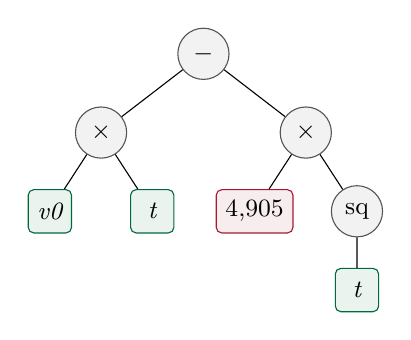
\begin{tikzpicture}[level distance=10mm,
          level 1/.style={sibling distance=26mm}, level 2/.style={sibling distance=13mm}]
        \node[op] {$-$}
          child { node[op] {$\times$} child { node[var] {v0} } child { node[var] {t} } }
          child { node[op] {$\times$} child { node[cst] {4,905} } child { node[op] {sq} child { node[var] {t} } } };
      \end{tikzpicture}\par\medskip
      \begin{itemize}\footnotesize
        \item węzeł zna tylko \textbf{nazwę} operatora; funkcja pochodzi z rejestru
        \item złożoność = liczba węzłów (jak w PySR)
      \end{itemize}
    \end{column}
  \end{columns}
\end{frame}

% ---------------------------------------------------------------------------- 5
\section{Etap 16.11: Weryfikacja MVP}
\begin{frame}{Etap 16.11: Optymalizacja stałych (\texttt{sr::optimize\_constants})}
  \begin{columns}[c]
    \begin{column}{0.44\textwidth}
      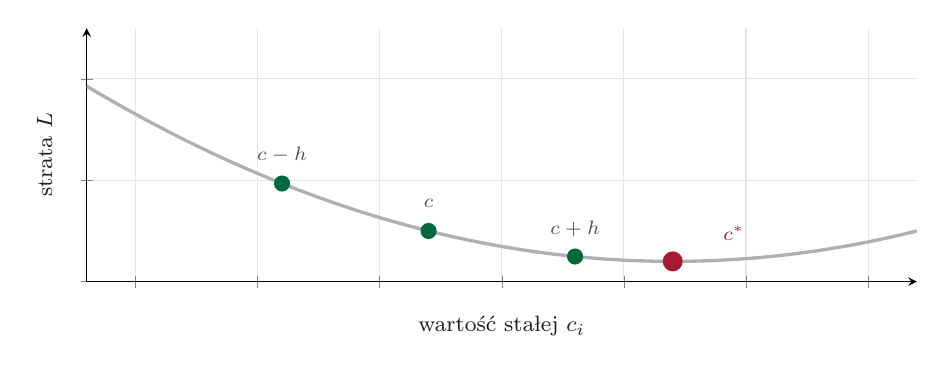
\begin{tikzpicture}
        \begin{axis}[srplot, xlabel={wartość stałej $c_i$}, ylabel={strata $L$},
            yticklabels={}, xticklabels={}, xmin=-0.2, xmax=3.2, ymin=0, ymax=5]
          \addplot[color=aghfaint, domain=-0.2:3.2, samples=60] {0.6*(x-2.2)^2 + 0.4};
          \addplot[only marks, mark=*, mark size=2.3pt, color=aghgreen] coordinates {(0.6,1.936) (1.2,1.0) (1.8,0.496)};
          \addplot[only marks, mark=*, mark size=3pt, color=aghred] coordinates {(2.2,0.4)};
          \node[font=\scriptsize, color=aghmuted] at (axis cs:0.6,2.5) {$c-h$};
          \node[font=\scriptsize, color=aghmuted] at (axis cs:1.2,1.55) {$c$};
          \node[font=\scriptsize, color=aghmuted] at (axis cs:1.8,1.05) {$c+h$};
          \node[font=\scriptsize, color=aghred] at (axis cs:2.45,0.95) {$c^*$};
        \end{axis}
      \end{tikzpicture}
    \end{column}
    \begin{column}{0.53\textwidth}
      \textbf{Przeszukiwanie kolejnych współrzędnych:}
      \begin{enumerate}\footnotesize
        \item oblicz $L(c_i + h_i)$ i $L(c_i - h_i)$
        \item jeśli wypukło, skocz do wierzchołka paraboli:\\
          $c^* = c_i - h_i\,\dfrac{L_+ - L_-}{2(L_+ - 2L_0 + L_-)}$
        \item przyjmij najlepszy punkt; brak poprawy $\Rightarrow h_i / 2$
      \end{enumerate}
      \begin{itemize}\footnotesize
        \item bez gradientów (zamiast BFGS) --- odporne na obszary $+\infty$
        \item stała liniowa przy MSE $\Rightarrow$ \textcolor{aghred}{\textbf{dokładnie w 1 kroku}}
        \item test: $a x + b$ z $(1,0) \to (2{,}5;\ 0{,}75)$ z błędem $< 10^{-9}$
        \item uruchamiane na $5\%$ potomków + na wpisach hall of fame
      \end{itemize}
    \end{column}
  \end{columns}
\end{frame}

% ---------------------------------------------------------------------------- 6
\begin{frame}{Etap 16.11: \texttt{sr::fit}, \texttt{sr::predict}, front Pareta i \texttt{sr\_search}}
  \begin{columns}[c]
    \begin{column}{0.48\textwidth}
      \begin{tikzpicture}
        \begin{axis}[srplot, ymode=log, xlabel={złożoność (węzły)}, ylabel={MSE (trening)},
            xmin=0, xmax=9, xtick={1,3,5,7}, ymin=1e-32, ymax=1e3, ytick={1e2,1e-8,1e-18,1e-28}]
          \addplot[const plot, color=aghgreen, mark=*, mark size=2pt] coordinates {
            (1, 21.621899060434455)
            (3, 12.784461604734364)
            (5, 4.8726805683133039)
            (7, 1.4686660273410966e-30)
          };
          \addplot[only marks, mark=o, mark size=5pt, color=aghred, line width=1.5pt]
            coordinates {(7, 1.4686660273410966e-30)};
          \node[font=\scriptsize, anchor=north] at (axis cs:1.4,4) {stała};
          \node[font=\scriptsize, anchor=north] at (axis cs:4.9,1.2) {$t(v_0 - 7{,}28)$};
          \node[font=\scriptsize, anchor=east] at (axis cs:6.6,1e-27) {$t(v_0 - 4{,}905\,t)$};
        \end{axis}
      \end{tikzpicture}\par
      {\scriptsize\color{aghmuted}Rzut pionowy bez szumu, ziarno 2 (dane rzeczywiste)}
    \end{column}
    \begin{column}{0.49\textwidth}
      \textbf{Endpointy MVP:}
      \begin{itemize}\footnotesize
        \item \texttt{sr::predict(expr, fn, data)} --- kompiluje drzewo raz do programu postfiksowego (zgodne z \texttt{evaluate} na 300 losowych drzewach)
        \item \texttt{sr::fit(train, val, opts, fn)} --- hall of fame (najlepszy wzór dla każdej złożoności) $\to$ front Pareta
        \item wybór na \textbf{walidacji}: najprostszy wzór o stracie $\le \max(1{,}05\,L_{\min},\ 10^{-12} L_1)$
        \item \textbf{CLI \texttt{sr\_search}:} eksport \texttt{hall\_of\_fame.csv}, \texttt{progress.csv}, \texttt{result.json}, \texttt{--trace}
        \item \texttt{SearchObserver}: rejestracja przebiegu bez wpływu na RNG
      \end{itemize}
    \end{column}
  \end{columns}
\end{frame}

% ---------------------------------------------------------------------------- 7
\section{Etap 23.11: Konfigurowalność i ograniczenia}
\begin{frame}[fragile]{Etap 23.11: Własne operatory i funkcja straty (\texttt{sr\_custom})}
  \begin{columns}[c]
    \begin{column}{0.56\textwidth}
\begin{lstlisting}
sr::FunctionRegistry functions;
functions.add_unary ("exp",
    [](double x) { return std::exp(x); });
functions.add_binary("hypot",
    [](double a, double b) { return std::hypot(a, b); });
functions.add_loss  ("huber", [](double p, double y) {
    const double e = std::abs(p - y);
    return e <= 1.0 ? 0.5 * e * e : e - 0.5;
});

sr::SearchOptions options;
options.unary_operators  = {"exp"};
options.binary_operators = {"+", "-", "*", "hypot"};
options.loss = "huber";   // petla zna tylko nazwy
const auto result = sr::fit(forces, options, functions);
\end{lstlisting}
    \end{column}
    \begin{column}{0.41\textwidth}
      \textbf{Wynik uruchomienia \texttt{sr\_custom}:}
      \begin{itemize}\footnotesize
        \item zadanie: wypadkowa sił $|F|$ z $(F_x, F_y)$
        \item znaleziono: \textcolor{aghgreen}{\textbf{\texttt{hypot(Fy, Fx)}}} (złożoność 3, strata Hubera = \textbf{0})
        \item pętla wyszukiwania \textbf{bez żadnych zmian}
      \end{itemize}
      \medskip
      \textbf{Walidacja i błędy:}
      \begin{itemize}\footnotesize
        \item \texttt{sr::validate()} odrzuca 27 błędnych konfiguracji przed startem (nieznana nazwa, zła arność, duplikat)
        \item wyjątek \texttt{domain\_error} w funkcji użytkownika (np. \texttt{exp(1000)}) $\Rightarrow$ strata $+\infty$
      \end{itemize}
    \end{column}
  \end{columns}
\end{frame}

% ---------------------------------------------------------------------------- 8
\begin{frame}{Etap 23.11: Ograniczenia złożoności (\texttt{sr::Constraints}, \texttt{sr::violation})}
  \begin{columns}[T]
    \begin{column}{0.37\textwidth}
      \textbf{Konfigurowalne limity:}
      \begin{itemize}\footnotesize
        \item \texttt{max\_size} --- maks. liczba węzłów
        \item \texttt{max\_depth} --- maks. głębokość
        \item \texttt{arguments[op]} --- maks. rozmiar każdego argumentu (jak \texttt{constraints} w PySR)
        \item \texttt{ExponentLimit} --- wykładnik \texttt{pow}: stała, $|e| \le k$, opcjonalnie całkowita
        \item \texttt{pow} bez ochrony: $(-8)^{1/3}$, $0^{-1}$, przepełnienie $\Rightarrow$ \texttt{domain\_error}
      \end{itemize}
    \end{column}
    \begin{column}{0.60\textwidth}
      \textbf{Komunikaty \texttt{sr::violation()} w \texttt{sr\_constraints}:}\par\smallskip
      \scriptsize
      \begin{tabular}{@{}l l@{}}
        \toprule
        Wyrażenie & Wynik reguły \\
        \midrule
        $t^2$ & \textcolor{aghgreen}{admissible} \\
        $t^{2{,}5}$ & \texttt{exponent 2.5 of pow must be an integer} \\
        $t^4$ & \texttt{exponent 4 of pow exceeds |3|} \\
        $t^t$ & \texttt{exponent of pow must be a constant} \\
        $(t + t\cdot t)^2$ & \texttt{argument 1 of pow has size 5 > 3} \\
        $\cos(2(t+1))$ & \texttt{argument 1 of cos has size 5 > 3} \\
        \bottomrule
      \end{tabular}
    \end{column}
  \end{columns}
\end{frame}

% ---------------------------------------------------------------------------- 9
\begin{frame}{Etap 23.11: Egzekwowanie limitów w wyszukiwaniu}
  \begin{columns}[T]
    \begin{column}{0.50\textwidth}
      \textbf{Trzy poziomy ochrony:}
      \begin{enumerate}\footnotesize
        \item \textbf{Z konstrukcji (\texttt{Variation::grow}):}
          generator dzieli budżet rozmiaru między argumenty, ucina do \texttt{ArgumentLimit}, a wykładnik losuje z dozwolonego zakresu.
        \item \textbf{Filtr po każdej wariacji:}
          \texttt{admissible()} = \texttt{violation()} + dozwolone operatory (z arnością) i zmienne; odrzucona propozycja $\Rightarrow$ powtórz (do 10$\times$), inaczej kopia rodzica.
        \item \textbf{Optymalizator stałych:}
          drzewo niedopuszczalne dostaje stratę $+\infty$, więc wykładnik nie opuści dozwolonego zbioru.
      \end{enumerate}
    \end{column}
    \begin{column}{0.46\textwidth}
      \textbf{Pomiar z \texttt{sr\_constraints}:}\par
      {\scriptsize\color{aghmuted}rzut pionowy, \texttt{max\_size} 11, \texttt{max\_depth} 5, \texttt{pow}: (3, 1), $|e|\le 3$ całkowity}\par\smallskip
      \footnotesize
      \begin{tabular}{@{}lr@{}}
        \toprule
        Metryka & Wartość \\
        \midrule
        utworzeni potomkowie & 3\,840 \\
        odrzucone propozycje & \textcolor{aghred}{\textbf{1\,144}} \\
        kopie rodzica po 10 próbach & 0 \\
        dopuszczalni na końcu & \textcolor{aghgreen}{\textbf{69 / 69}} \\
        \bottomrule
      \end{tabular}\par\medskip
      {\scriptsize Test własności: $10 \text{ ziaren} \times 4\,000 \text{ kroków}$ --- każdy potomek dopuszczalny, a część surowych propozycji narusza limity.}
    \end{column}
  \end{columns}
\end{frame}

% ---------------------------------------------------------------------------- 10
\section{Wyniki, testy i dalsze prace}
\begin{frame}{Wstępne wyniki i przypadek nieudany (budżet 1--4 s)}
  \begin{columns}[c]
    \begin{column}{0.52\textwidth}
      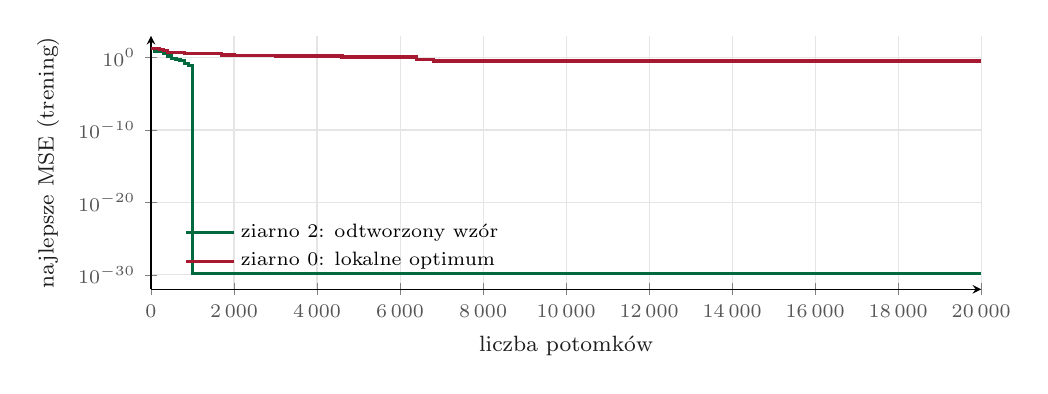
\begin{tikzpicture}
        \begin{axis}[srplot, ymode=log, xlabel={liczba potomków}, ylabel={najlepsze MSE (trening)},
            xmin=0, xmax=20000, ymin=1e-32, ymax=1e3, ytick={1e0,1e-10,1e-20,1e-30},
            scaled x ticks=false, xticklabel style={/pgf/number format/1000 sep={\,}},
            legend pos=south west]
          \addplot[const plot, color=aghgreen] coordinates {
            (0,17.7124) (100,6.61044) (200,6.61044) (300,3.90082) (400,1.70371)
            (500,0.806396) (600,0.585727) (700,0.406436) (800,0.141373) (900,0.0839309)
            (1000,1.46867e-30) (20000,1.46867e-30)
          };
          \addlegendentry{ziarno 2: odtworzony wzór}
          \addplot[const plot, color=aghred] coordinates {
            (0,17.0471) (100,16.8502) (200,13.5220) (300,9.84199) (400,5.48587)
            (500,4.92702) (600,4.91721) (800,3.97760) (1000,3.80577) (1500,3.30911)
            (1700,2.21614) (2000,1.80233) (3000,1.69762) (4500,1.62129) (4600,1.23742)
            (5800,1.14647) (6400,0.495134) (6800,0.347367) (8000,0.333375) (10000,0.331215)
            (13700,0.331086) (20000,0.331086)
          };
          \addlegendentry{ziarno 0: lokalne optimum}
        \end{axis}
      \end{tikzpicture}
    \end{column}
    \begin{column}{0.45\textwidth}
      \footnotesize
      \begin{tabular}{@{}llcc@{}}
        \toprule
        Zależność & Wariant & Odtw. & Złoż. \\
        \midrule
        sprężyna & bez / z szumem & 3/3, 3/3 & 5 \\
        rzut pionowy & bez / z szumem & 1/3, 2/3 & 7 \\
        oscylator & bez / z szumem & 2/3, 1/3 & 8--9 \\
        \bottomrule
      \end{tabular}\par\medskip
      \textbf{Obserwacje (18 uruchomień):}
      \begin{itemize}\footnotesize
        \item jedna populacja może utknąć w lokalnym optimum (PySR: 31 wysp)
        \item brak upraszczania: $t+(t+c)$ zamiast $2t+c$
        \item przy budżecie 15 s odtworzono 3 z 5 wcześniejszych porażek
      \end{itemize}
    \end{column}
  \end{columns}
\end{frame}

% ---------------------------------------------------------------------------- 11
\begin{frame}{Testy automatyczne i dalsze prace}
  \begin{columns}[T]
    \begin{column}{0.52\textwidth}
      \textbf{Weryfikacja (\texttt{ctest} --- 7 celów, 0 ostrzeżeń):}
      \begin{itemize}\footnotesize
        \item \texttt{sr\_tests} --- CSV, dane fizyczne, drzewa, własne operatory i straty
        \item \texttt{sr\_search\_tests} --- edycja preorder, \texttt{pow} i przypadki brzegowe, każda reguła ograniczeń \textbf{na granicy i krok za nią}, 27 błędnych konfiguracji, własności wariacji (10 ziaren), \texttt{optimize\_constants}, determinizm, \texttt{SearchObserver}, własne funkcje w wyszukiwaniu
        \item przechodzi w Debug, Release i pod ASan + UBSan
      \end{itemize}
    \end{column}
    \begin{column}{0.45\textwidth}
      \textbf{Następne etapy harmonogramu:}
      \begin{itemize}\footnotesize
        \item \textbf{30.11:} stały szablon wyrażenia z jednym uczonym poddrzewem, jawne listy zmiennych, narzędzie pomiarowe, zamrożenie konfiguracji
        \item \textbf{07.12:} 36 uruchomień porównawczych C++ vs PySR (90 s, 1 wątek) + mikropomiar
        \item \textbf{14.12:} końcowy raport LaTeX + instrukcja odtworzenia
        \item \textbf{21.12:} prezentacja końcowa i oddanie
      \end{itemize}
    \end{column}
  \end{columns}
\end{frame}

% ---------------------------------------------------------------------------- 12
\begin{frame}
  \centering\vfill
  {\LARGE\bfseries Dziękuję za uwagę. Pytania?}\par\bigskip
  {\small\color{aghmuted}
    Repozytorium: kod źródłowy, testy (\texttt{sr\_tests}, \texttt{sr\_search\_tests}),\\
    programy demo (\texttt{sr\_search}, \texttt{sr\_custom}, \texttt{sr\_constraints}) oraz wizualizator offline (\texttt{visualizer.html}).}
  \vfill
\end{frame}

\end{document}
